\documentclass[UTF8]{ctexart}
\usepackage{tabularx,makecell,multirow,diagbox}
\usepackage{graphicx}
\usepackage{float}
\usepackage{tikz}
\usetikzlibrary{automata, positioning, arrows}


\begin{document}

\section{对于线程的词法规则其概括性的DFA}
% 有限状态机
\centering
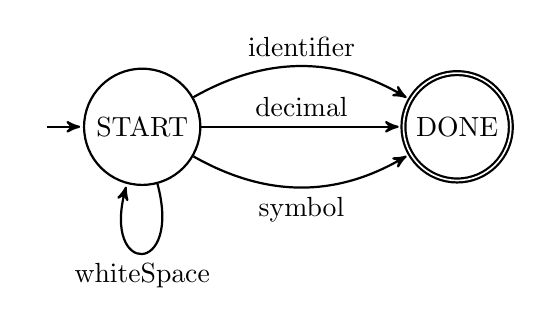
\begin{tikzpicture}[->,>=stealth',shorten >=1pt,auto,node distance=4cm,
    thick,base node/.style={circle,draw,minimum size=16pt}, real node/.style={double,circle,draw,minimum size=35pt}]

\node[initial,initial text={}, state]   (1)                     {START};
\node[state,accepting]                  (2)     [right of=1 ]   {DONE}          [above];

\path[]
(1) edge[loop below]node {whiteSpace} (1)
(1) edge[bend left,above] node{identifier} (2)
(1) edge[bend right, below] node{symbol} (2)
(1) edge  node{decimal} (2);
\end{tikzpicture}

其中whiteSpace表示为:空白,换行符和制表符,identifier表示可识别的标识符,decimal表示浮点数,symbol表示专用符号。

\section{将identifier,decimal,symbol分别拆开绘制DFA}

\subsection{identifier的DFA表示}
\subsubsection{identifier正规表达式的定义:}
\begin{verbatim}
identifier = identifier_letter (underline?letter_or_digit)*
identifier_letter=a|..|z|A|..|Z|
letter_or_digit = identifier_letter | digit
digit = 0|..|9
underline=_
\end{verbatim}
\subsubsection{identifier的NFA表示}
根据identifier的正规表达式对应的NFA的表示
% 有限状态机
\centering
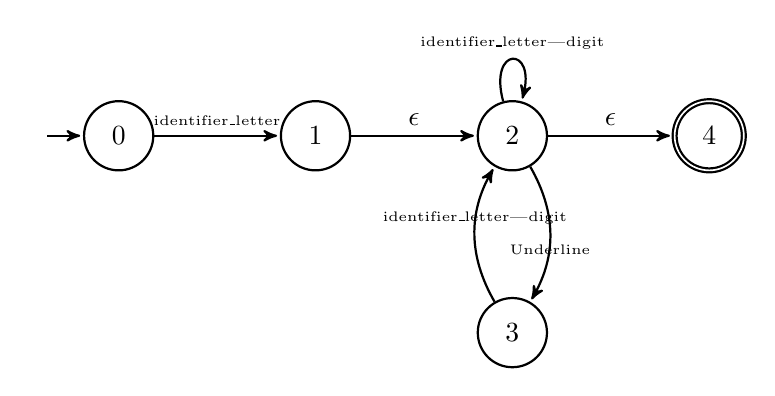
\begin{tikzpicture}[->,>=stealth',shorten >=1pt,auto,node distance=2.5cm,
    thick,base node/.style={circle,draw,minimum size=16pt}, real node/.style={double,circle,draw,minimum size=35pt}]

\node[initial,initial text={}, state]   (0)                     {0};
\node[state]                  (1)     [right of=0 ]   {1}          [above];
\node[state]                  (2)     [right of=1 ]   {2}          [above];
\node[state]                  (3)     [below of=2 ]   {3}          [above];
\node[state,accepting]        (4)     [right of=2 ]   {4}          [above];

\path[]
(0) edge node{\tiny{identifier\_letter}} (1)
(1) edge node{$\epsilon$} (2)
(2) edge[loop above] node{\tiny{identifier\_letter|digit}} (2)
(2) edge[bend left, below] node{\tiny{Underline}} (3)
(3) edge[bend left, above] node{\tiny{identifier\_letter|digit}} (2)
(2) edge  node{$\epsilon$} (4);
\end{tikzpicture}


\subsubsection{求解上述的$\varepsilon$-闭包}
$\overline{0}=\{ 0 \}$ 

$\overline{1}=\{ 1,2,4 \}$ 

$\overline{2}=\{ 2,4 \}$ 

$\overline{3}=\{ 3 \}$ 

$\overline{4}=\{ 4 \}$ 


\begin{tabular}{|c|c|c|c|}
\hline
\diagbox{状态}{输入} & identifier\_letter  & underline & digit \\
\hline
 \{0\} & \{1,2,4 \} & $\emptyset$ & $\emptyset$ \\
 \hline
 \{1,2,4\} & \{2,4\} & \{3\} &\{2,4\} \\
 \hline
 \{2,3,4\} &\{2,4\} & \{3\} & \{2,4\}\\ 
\hline

\end{tabular}

\subsubsection{identifier的DFA表示}
由上述的$\varepsilon$-闭包可得下述 identifier对应的DFA的表示
% 有限状态机
\centering
\begin{tikzpicture}[->,>=stealth',shorten >=1pt,auto,node distance=5cm,
    thick,base node/.style={circle,draw,minimum size=16pt}, real node/.style={double,circle,draw,minimum size=35pt}]

\node[initial,initial text={}, state]   (0)                     {0};
\node[state,accepting]        (2)     [right of=1 ]   {2}          [above];
\node[state]                  (1)     [below of=2 ]   {1}          [above];

\path[]
(0) edge node{identifier\_letter} (2)
(2) edge[bend right, below] node{underline} (1)
(1) edge[bend right, above] node{letter\_or\_digit} (2)
(2) edge[loop above] node{identifier\_letter|digit} (2);
\end{tikzpicture}


\subsection{decimal的DFA表示}
\subsubsection{decimal的正规表达式表示}
\begin{verbatim}
decimal = sign? numeral . numeral
numeral= digit (digit)*
sign = + | -
\end{verbatim}

\subsubsection{decimal的NFA表示}
decimal的NFA表示如下所示
% 有限状态机
\centering
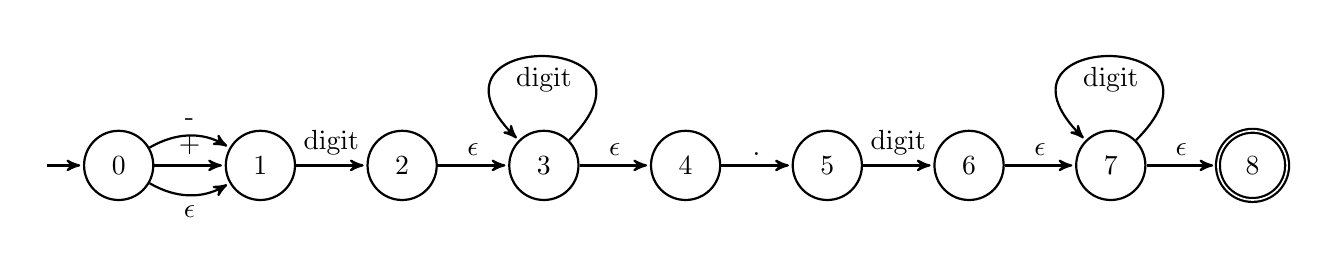
\begin{tikzpicture}[->,>=stealth',shorten >=1pt,auto,node distance=1.8cm,
    thick,base node/.style={circle,draw,minimum size=16pt}, real node/.style={double,circle,draw,minimum size=35pt}]

\node[initial,initial text={}, state]   (0)           {0};
\node[state]                  (1)     [right of=0 ]   {1};
\node[state]                  (2)     [right of=1 ]   {2};
\node[state]                  (3)     [right of=2 ]   {3};
\node[state]                  (4)     [right of=3 ]   {4};
\node[state]                  (5)     [right of=4 ]   {5};
\node[state]                  (6)     [right of=5 ]   {6};
\node[state]                  (7)     [right of=6 ]   {7};
\node[state,accepting]        (8)     [right of=7 ]   {8};

\path[]
(0) edge[bend left, above] node{-} (1)
(0) edge node{+} (1)
(0) edge[bend right, below] node{$\epsilon$} (1)
(1) edge node{digit} (2)
(2) edge node{$\epsilon$} (3)
(3) edge[loop, below] node{digit} (3)
(3) edge node{$\epsilon$} (4)
(4) edge node{$.$} (5)
(5) edge node{digit} (6)
(6) edge node{$\epsilon$} (7)
(7) edge[loop, below] node{digit} (7)
(7) edge node{$\epsilon$} (8)
;
\end{tikzpicture}

% \begin{figure}[htbp]
% \centering
% \includegraphics[scale=0.4]{NFADecimal.png}
% \label{fig:picture}
% \end{figure}


\subsubsection{求解上述的$\varepsilon$-闭包}

$\overline{0}=\{ 0,1 \}$ 

$\overline{1}=\{ 1,2 \}$ 

$\overline{2}=\{ 2,3,4 \}$ 

$\overline{3}=\{ 3,4 \}$ 

$\overline{4}=\{ 4 \}$ 

$\overline{5}=\{ 5 \}$ 

$\overline{6}=\{ 6,7,8 \}$ 

$\overline{7}=\{ 7,8 \}$ 

$\overline{8}=\{ 8 \}$ 


\begin{tabular}{|c|c|c|c|c|}
\hline
\diagbox{状态}{输入} & -  & + & digit & .\\
\hline
 \{0\} & \{1 \} &   \{1 \}  & $\emptyset$ & $\emptyset$  \\
 \hline
 \{1\} & $\emptyset$ & $\emptyset$ &\{2,3,4\}  & $\emptyset$ \\
 \hline
 \{2,3,4\} &$\emptyset$ &$\emptyset$ & \{3,4\}\ & \{5\}\\ 
\hline
 \{3,4,5\} &$\emptyset$ &$\emptyset$ & \{3,4,6,7,8\}\ & \{5\}\\ 
\hline
\{3,4,5,6,7,8\} &$\emptyset$ &$\emptyset$ & \{3,4,6,7,8\}\ & \{5\}\\ 
\hline
\end{tabular}

\subsubsection{decimal的DFA表示}
根据上述的$\varepsilon$-闭包可得下述decimal的DFA表示
% 有限状态机
\centering
\begin{tikzpicture}[->,>=stealth',shorten >=1pt,auto,node distance=1.8cm,
    thick,base node/.style={circle,draw,minimum size=16pt}, real node/.style={double,circle,draw,minimum size=35pt}]

\node[initial,initial text={}, state]   (0)           {0};
\node[state]                  (1)     [right of=0 ]   {1};
\node[state]                  (2)     [right of=1 ]   {2};
\node[state]                  (4)     [right of=2 ]   {4};
\node[state, accepting]       (5)     [right of=4 ]   {5};

\path[]
(0) edge[bend left, above] node{-} (1)
(0) edge[bend right, above] node{+} (1)
(0) edge[bend right, below] node{digit} (2)
(1) edge node{digit} (2)
(2) edge[loop, below] node{digit} (2)
(2) edge node{$\.$} (4)
(4) edge node{digit} (5)
(5) edge[loop, below] node{digit} (5)
;
\end{tikzpicture}

\subsection{symbol的DFA表示}
特殊符号的DFA表示如下所示
% 有限状态机
\centering
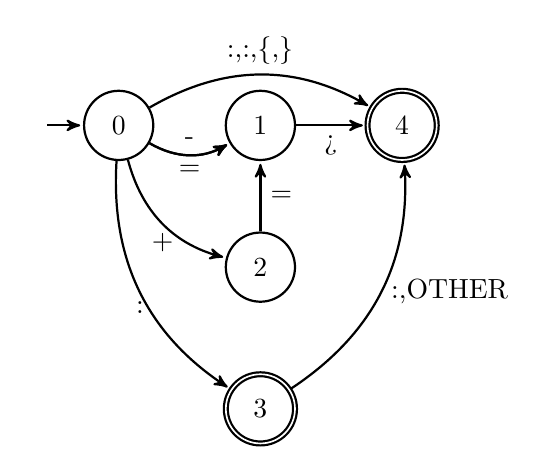
\begin{tikzpicture}[->,>=stealth',shorten >=1pt,auto,node distance=1.8cm,
    thick,base node/.style={circle,draw,minimum size=16pt}, real node/.style={double,circle,draw,minimum size=35pt}]

\node[initial,initial text={}, state]   (0)           {0};
\node[state]                  (1)     [right of=0 ]   {1};
\node[state]                  (2)     [below of=1 ]   {2};
\node[state,accepting]        (3)     [below of=2 ]   {3};
\node[state, accepting]       (4)     [right of=1 ]   {4};

\path[]
(0) edge[bend left, above] node{:,:,\{,\}} (4)
(0) edge[bend right, below] node{=} (1)
(0) edge[bend right, above] node{-} (1)
(0) edge[bend right, below] node{+} (2)
(0) edge[bend right, below] node{:} (3)
(2) edge[below, right=0.1] node{=} (1)
(1) edge[below] node{>} (4)
(3) edge[bend right, below, right=0.1] node{:,OTHER} (4)

;
\end{tikzpicture}
\section{整合后的DFA的表示}
因为特殊符号中与decimal有重复部分$+,-$,需要将二者拼接,最后的结果如下所示

% 有限状态机
\centering
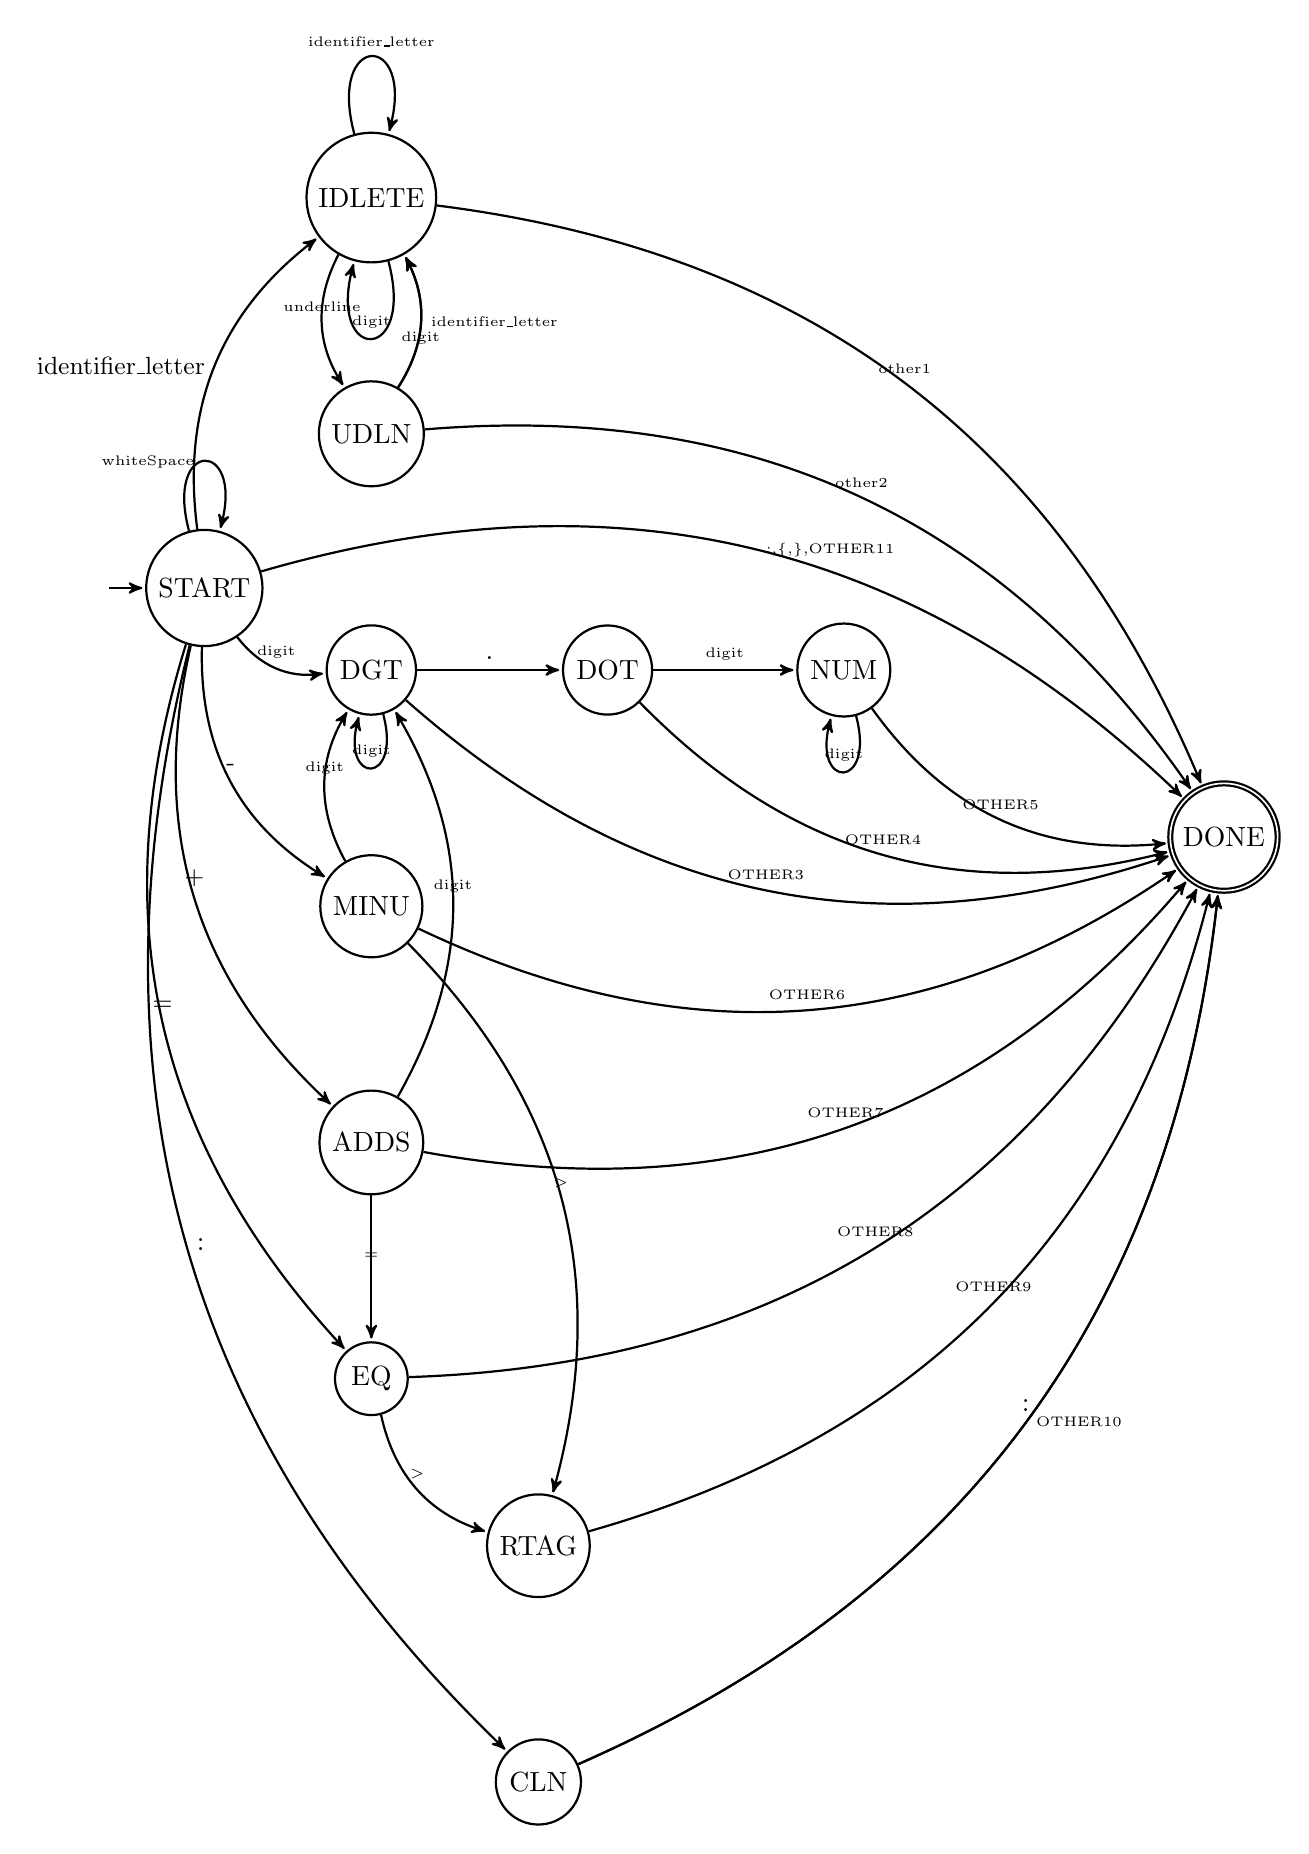
\begin{tikzpicture}[->,>=stealth',shorten >=1pt,auto,node distance=3cm,
    thick,base node/.style={circle,draw,minimum size=10pt}, real node/.style={double,circle,draw,minimum size=25pt}]

\node[initial,initial text={}, state]   (START)           {START};
\node[state]                  (IDLETE)     [above right of=START, above = 2 ]   {IDLETE};
\node[state]                  (UDLN)     [below of=IDLETE ]   {UDLN};
\node[state]                  (DGT)     [below of=UDLN ]   {DGT};
\node[state]                  (DOT)     [right of=DGT ]   {DOT};
\node[state]                  (NUM)     [right of=DOT ]   {NUM};
\node[state]                  (MINU)     [below of=DGT ]   {MINU};
\node[state]                  (ADDS)     [below of=MINU ]   {ADDS};
\node[state]                  (EQ)     [below of=ADDS ]   {EQ};
\node[state]                  (RTAG)     [below right of= EQ ]   {RTAG};
\node[state]                  (CLN)     [below of=RTAG ]   {CLN};
\node[state, accepting]       (DONE)     [below right of=NUM, right=2 ]   {DONE};

\path[]
(START) edge[bend left, above, left=1] node{\small{identifier\_letter}} (IDLETE)
(START) edge[loop above, below, left = 1] node{\tiny{whiteSpace}} (START)
(START) edge[bend right, above] node{\tiny{digit}} (DGT)
(START) edge[bend right, above] node{\small{-}} (MINU)
(START) edge[bend right, above] node{\small{+}} (ADDS)
(START) edge[bend right, above] node{\small{=}} (EQ)
(START) edge[bend right, above, right=1] node{:} (CLN)
(START) edge[bend left, above, right=1] node{\tiny{:,\{,\},OTHER11}} (DONE)

(IDLETE) edge[loop above, above] node{\tiny{identifier\_letter}} (IDLETE)
(IDLETE) edge[loop below, above] node{\tiny{digit}} (IDLETE)
(IDLETE) edge[bend right, above] node{\tiny{underline}} (UDLN)
(IDLETE) edge[bend left, above] node{\tiny{other1}} (DONE)

(UDLN) edge[bend right, above, right=1] node{\tiny{identifier\_letter}} (IDLETE)
(UDLN) edge[bend right, below] node{\tiny{digit}} (IDLETE)
(UDLN) edge[bend left, above] node{\tiny{other2}} (DONE)

(CLN) edge[bend right, above] node{:} (DONE)
(CLN) edge[bend right, below, right=1] node{\tiny{OTHER10}} (DONE)

(DGT) edge node{.} (DOT)
(DGT) edge[bend right, above] node{\tiny{OTHER3}} (DONE)
(DGT) edge[loop below, above] node{\tiny{digit}} (DGT)

(DOT) edge node{\tiny{digit}} (NUM)
(DOT) edge[bend right, above] node{\tiny{OTHER4}} (DONE)

(NUM) edge[loop below, above] node{\tiny{digit}} (NUM)
(NUM) edge[bend right, above] node{\tiny{OTHER5}} (DONE)

(MINU) edge[bend left, above] node{\tiny{digit}} (DGT)
(MINU) edge[bend right, above] node{\tiny{OTHER6}} (DONE)
(MINU) edge[bend left, above] node{\tiny{>}} (RTAG)

(ADDS) edge[bend right, above] node{\tiny{digit}} (DGT)
(ADDS) edge[above] node{\tiny{=}} (EQ)
(ADDS) edge[bend right, above] node{\tiny{OTHER7}} (DONE)

(EQ) edge[bend right, above] node{\tiny{>}} (RTAG)
(EQ) edge[bend right, above] node{\tiny{OTHER8}} (DONE)

(RTAG) edge[bend right, above] node{\tiny{OTHER9}} (DONE)

;
\end{tikzpicture}
% \begin{figure}[htbp]
% \centering
% \includegraphics[scale=0.4]{DFA.png}
% \label{fig:picture}
% \end{figure}

OTHER1表示:除identifier\_letter,digit之外的字符

OTHER2表示:除underline,identifier\_letter,digit之外的字符

OTHER3表示:除digit之外的字符

OTHER4表示:除digit之外的字符

OTHER5表示:任意字符

OTHER6表示:除digit,>之外的字符

OTHER7表示:除digit,=之外的字符

OTHER8表示:除>之外的字符

OTHER9表示:任意字符

OTHER10表示:除:之外的字符

OTHER11表示:除;,\{,\}之外的字符
\end{document}